\documentclass{ethpresentation}

\begin{document}
  \maketitle
  % \section{First Section}
  \begin{frame}{Our goal is a functioning low-field\\NMR benchtop spectrometer}
    \begin{figure}
      \centering
      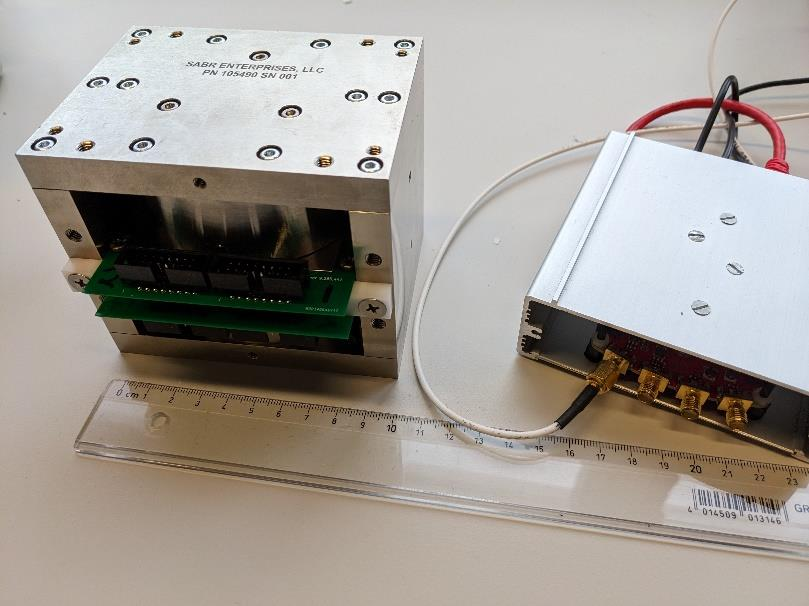
\includegraphics[width=\textwidth,height=0.8\textheight,keepaspectratio]{./img/magnet.png}
    \end{figure}
  \end{frame}
  \begin{frame}{We've made a probe holder\\and an RF-coil already}
    \begin{columns}
      \begin{column}{0.45\textwidth}
        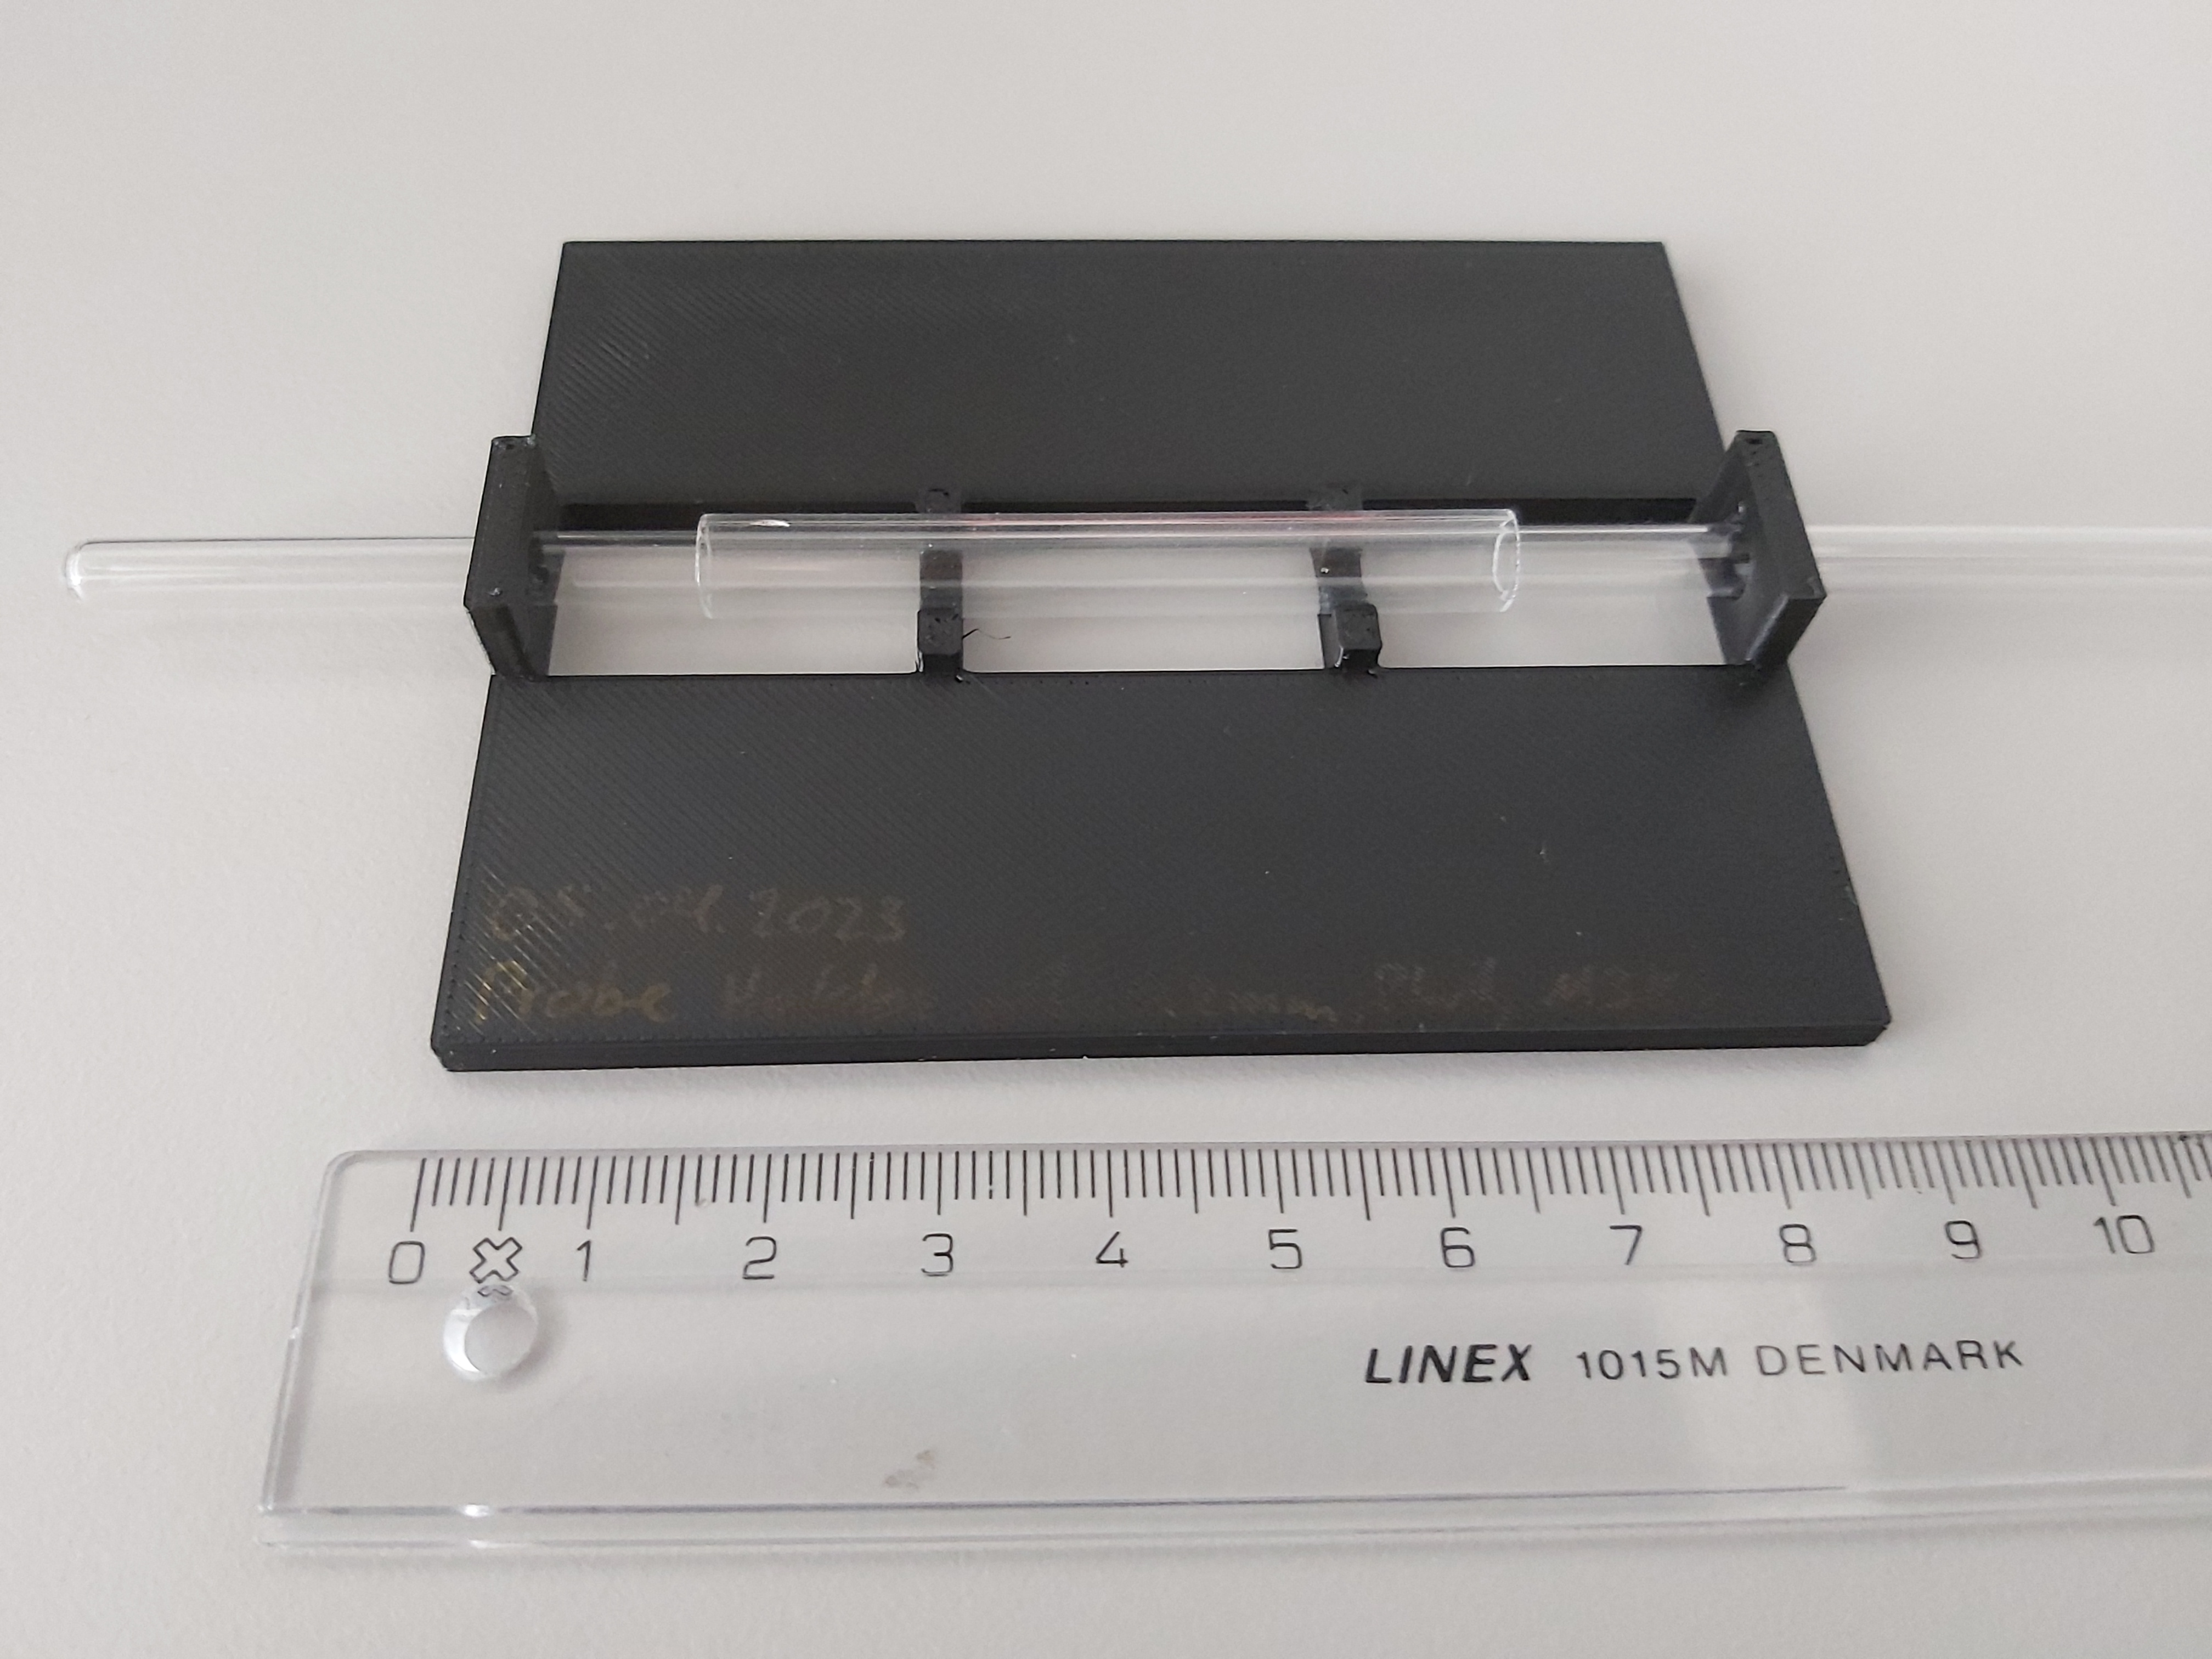
\includegraphics[width=\textwidth]{./img/probe_holder.jpg}
      \end{column}
      \begin{column}{0.45\textwidth}
        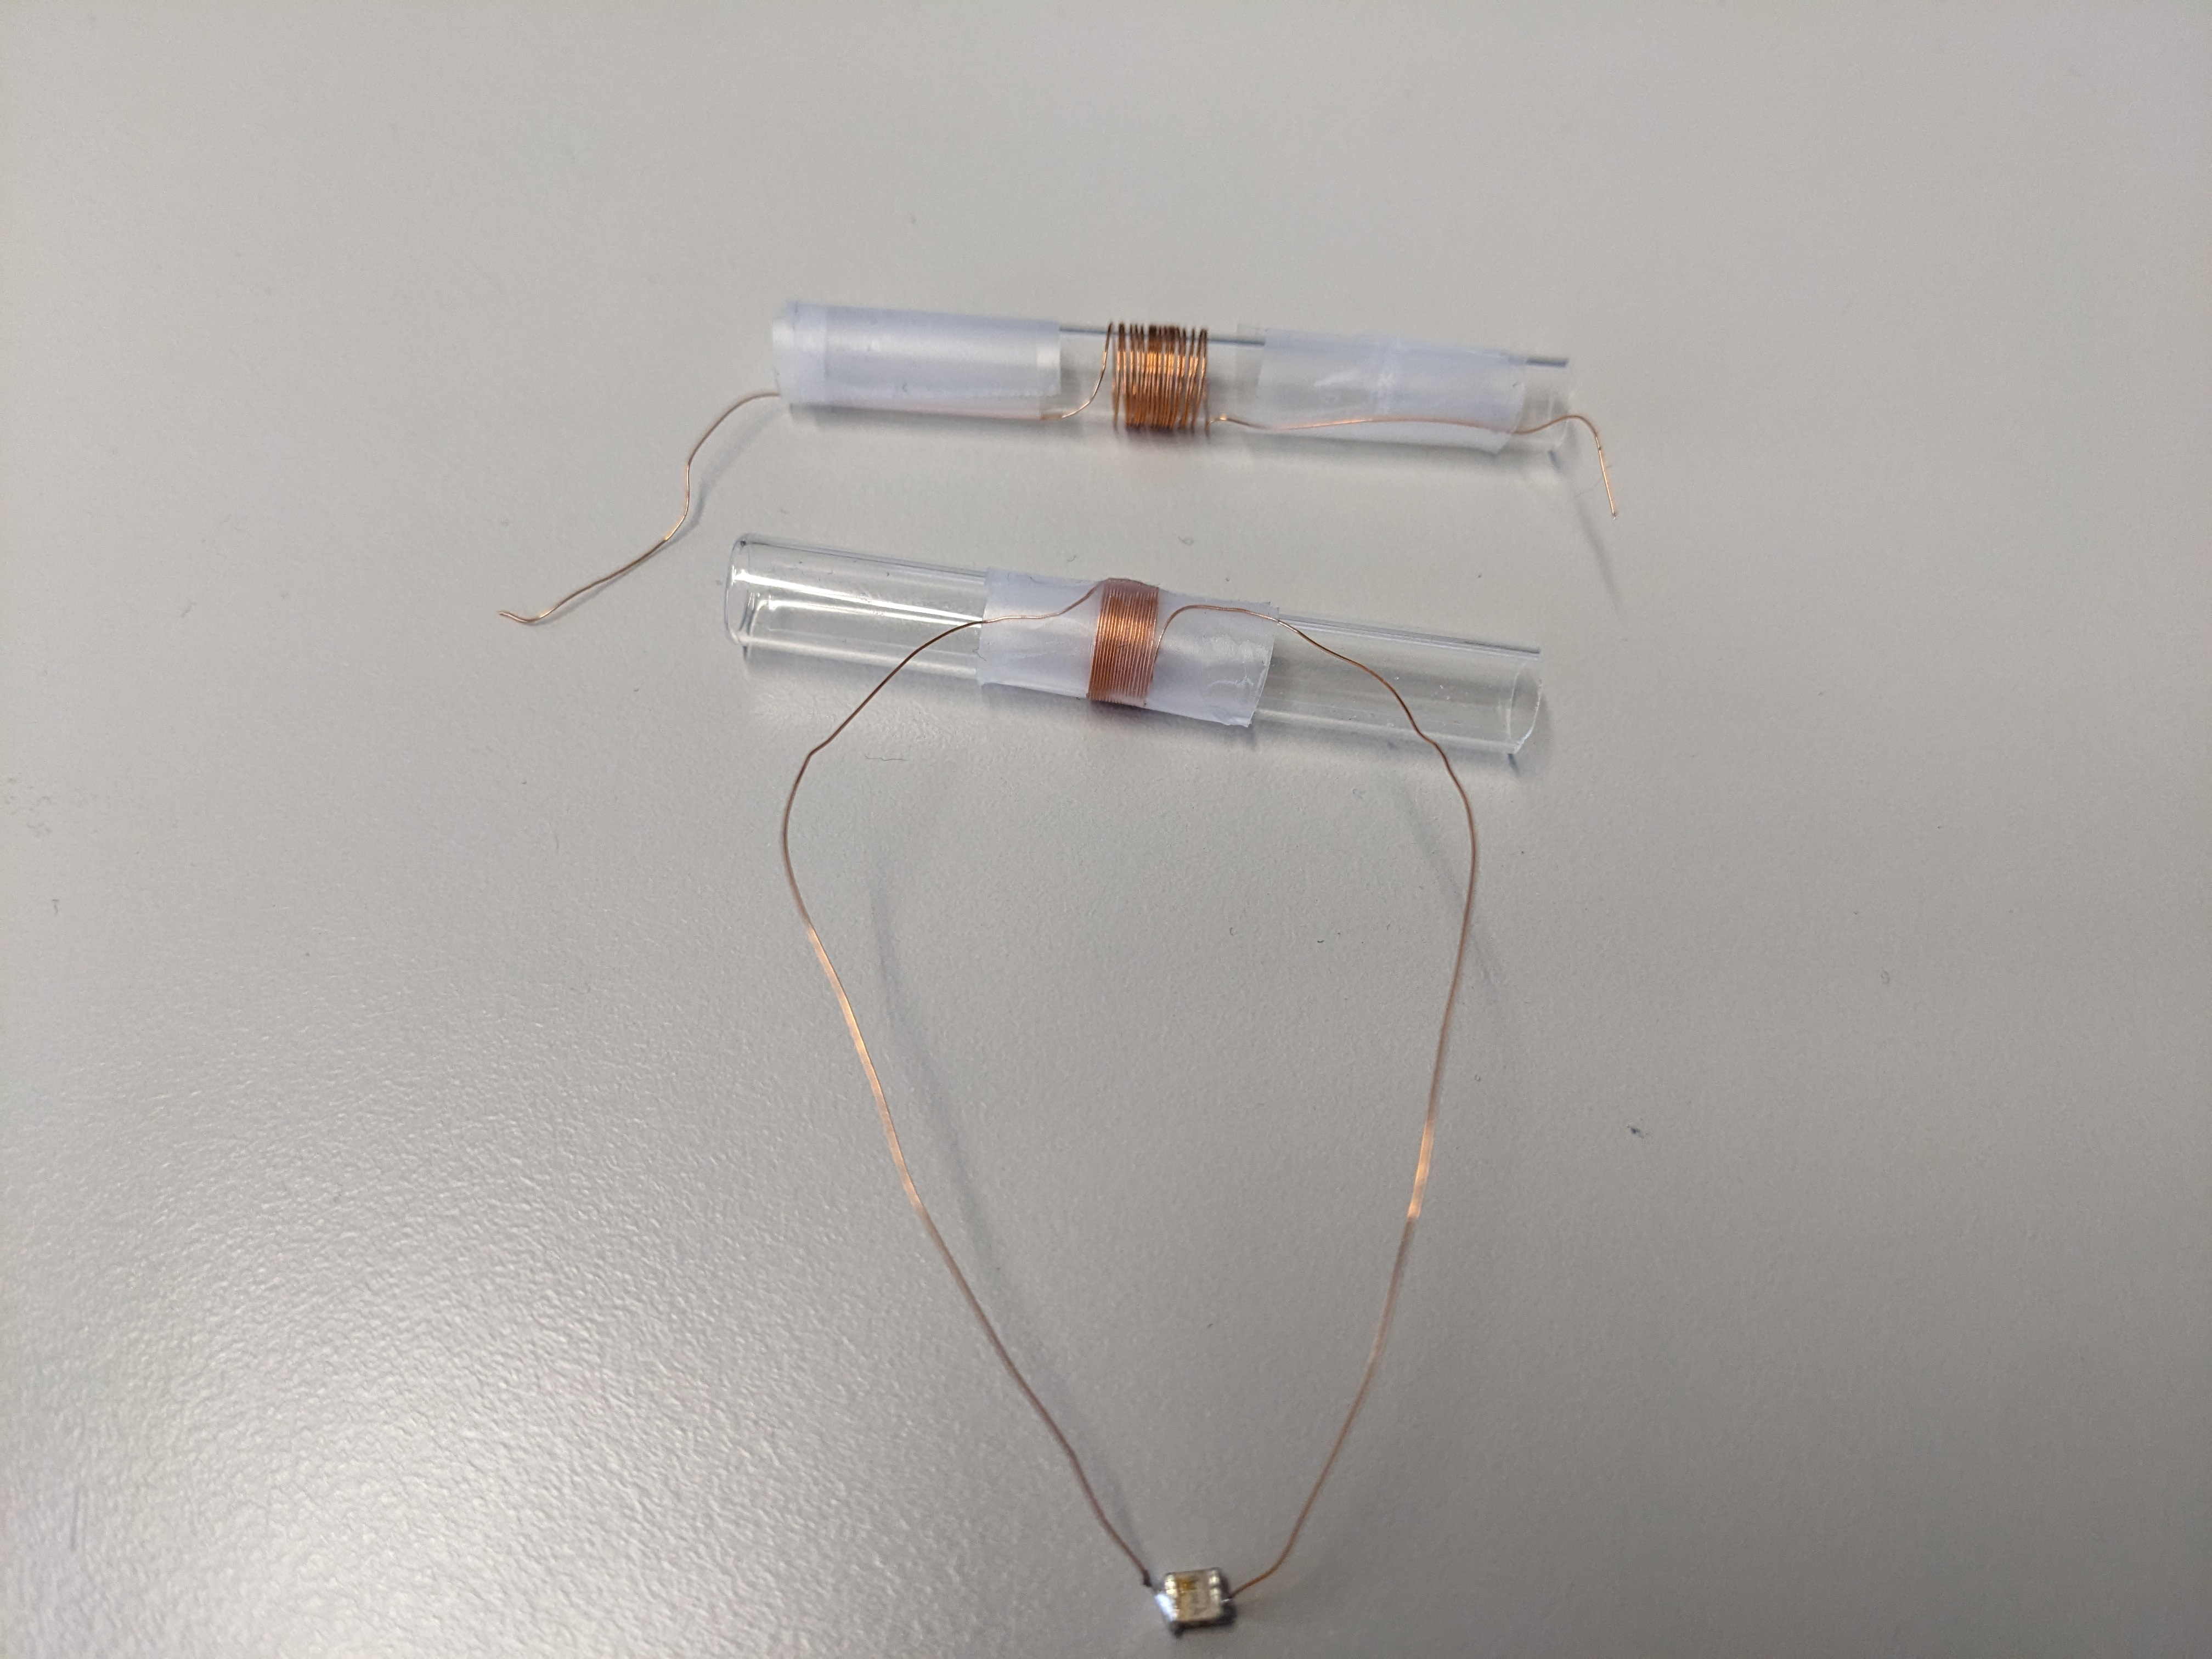
\includegraphics[width=\textwidth]{./img/coil.jpg}
      \end{column}
    \end{columns}
  \end{frame}
  \begin{frame}{Next we will setup the console, measure the magnetic field\\and build, match and tune the probe}
    \begin{columns}
      \begin{column}{0.33\textwidth}
        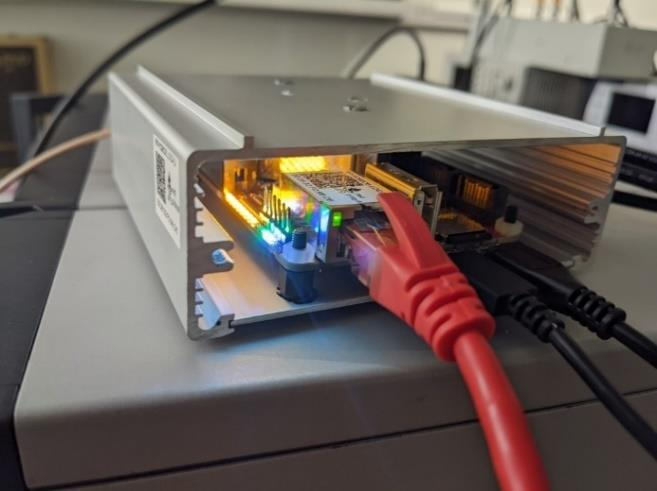
\includegraphics[width=\textwidth, height=0.8\textheight, keepaspectratio]{./img/red_pitaya.png}
      \end{column}
      \begin{column}{0.33\textwidth}
        \centering
        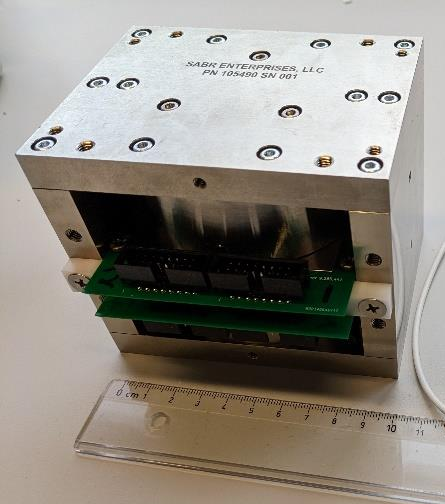
\includegraphics[width=\textwidth, height=0.8\textheight, keepaspectratio]{./img/magnet_only.png}
      \end{column}
      \begin{column}{0.33\textwidth}
        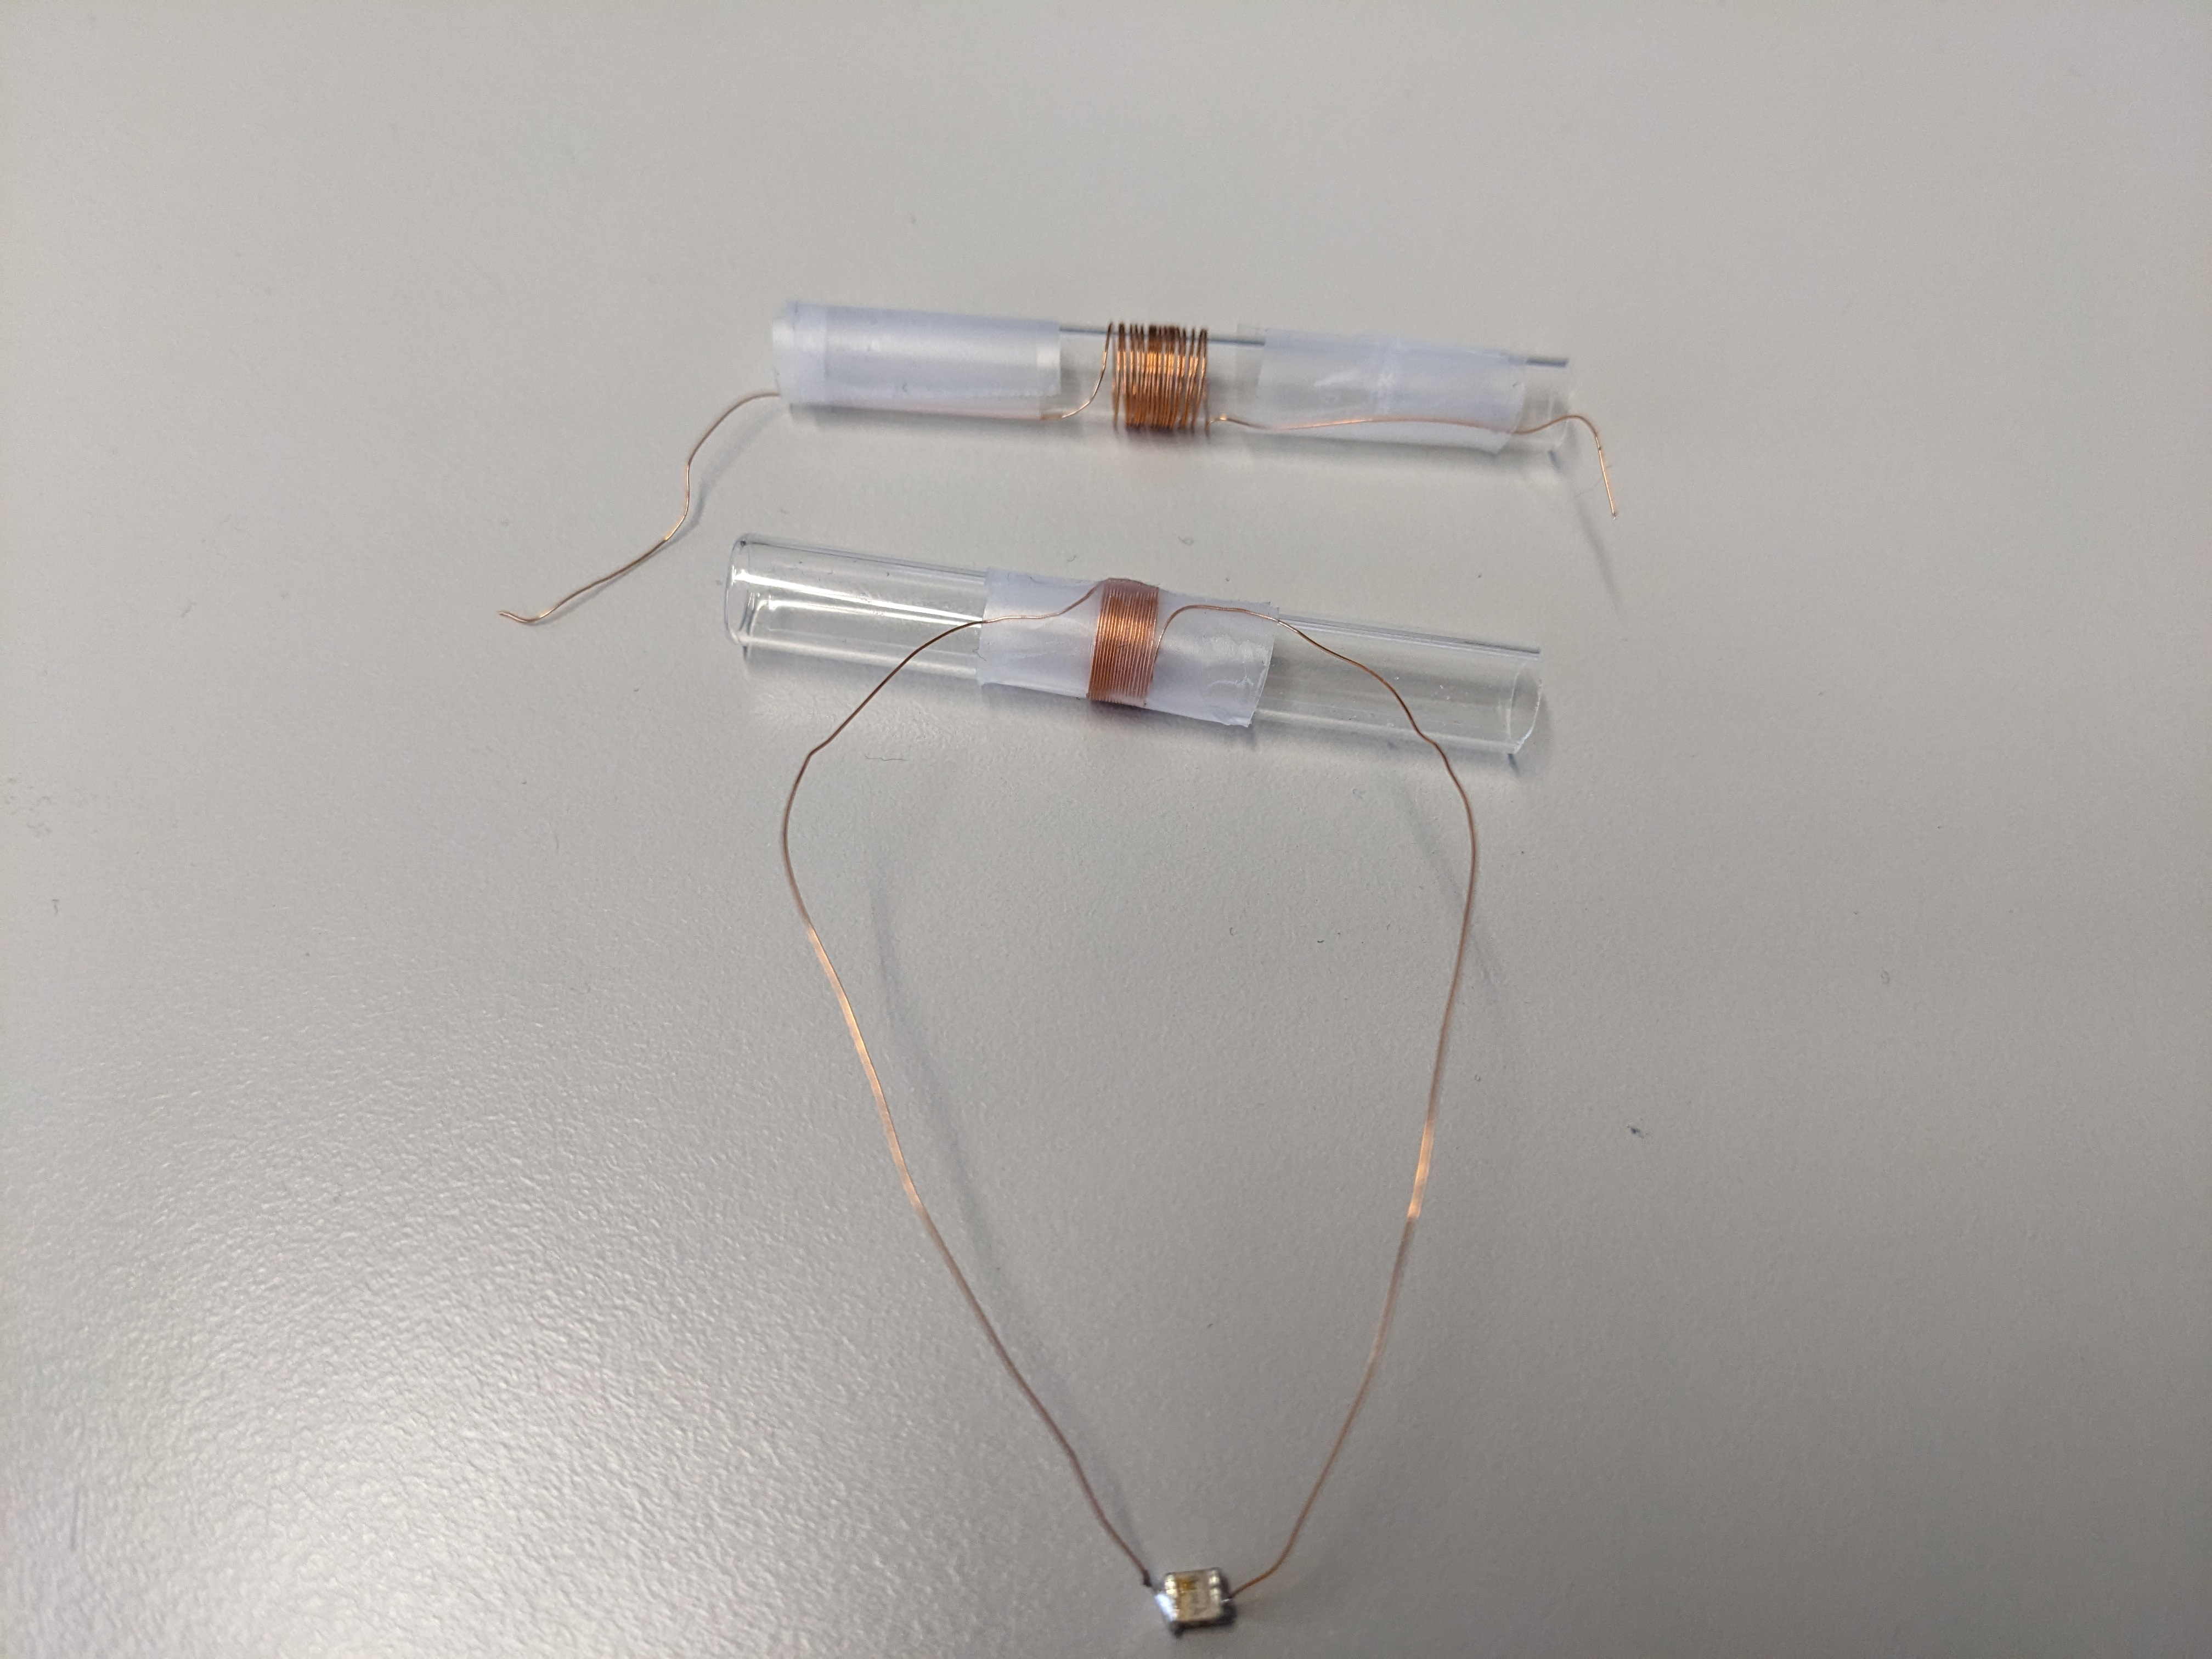
\includegraphics[width=\textwidth, height=0.8\textheight, keepaspectratio]{./img/coil.jpg}
      \end{column}
    \end{columns}
  \end{frame}
  \begin{frame}[standout]
    Thank you!
  \end{frame}
  \appendix
  % \begin{frame}[standout]
  %   A backup graph for explaining things.
  % \end{frame}
\end{document}